\chapter{Datasets, Backbones and Evaluation Protocol}
\label{ch:data}

This chapter fixes the experimental ground: the datasets and their splits, the OOD sets, the two
backbones, the episodic protocol, and the metrics.

\section{Datasets}
\label{sec:datasets}

\subsection{In-distribution datasets}

Both datasets use the standard 64/16/20 class split: 64 classes for training the adapter, 16 for
validation and 20 held out for testing. The three groups of classes are disjoint, so test accuracy
measures generalisation to classes the adapter has never seen.

\begin{itemize}
\item \textbf{CIFAR-FS}~\cite{bertinetto2019r2d2}: the 100 classes of CIFAR-100~\cite{krizhevsky2009cifar}
($32 \times 32$ images), split 64/16/20.
\item \textbf{MiniImageNet}~\cite{vinyals2016matching}: 100 ImageNet classes stored at $84 \times 84$,
with the split of Ravi and Larochelle~\cite{ravi2017optimization}.
\end{itemize}

The backbones were pretrained at $224 \times 224$, so every image is resized to $224 \times 224$ and
normalised with the ImageNet mean and standard deviation. No data augmentation is used. The class splits
are stored as fixed files and never regenerated.

\subsection{Out-of-distribution sets}

Each in-distribution dataset is evaluated against four OOD sets of 500 images each, drawn once with a
fixed seed and preprocessed in the same way:

\begin{itemize}
\item \textbf{SVHN}~\cite{netzer2011svhn} (far-OOD): street-view house-number digits from the SVHN test
set, unrelated to the natural-image classes.
\item \textbf{Gaussian noise} (far-OOD): images of independent standard normal noise, the simplest
possible OOD input.
\item \textbf{Held-out classes} (near-OOD): 500 images from the 16 validation classes of the same
dataset, i.e.\ held-out CIFAR-100 classes for CIFAR-FS and held-out MiniImageNet classes for
MiniImageNet. These share the visual domain of the in-distribution data but are never test classes.
\item \textbf{TinyImageNet}~\cite{le2015tinyimagenet} (near-OOD): images from the TinyImageNet training
partition. For MiniImageNet, the 25 TinyImageNet classes that also appear among MiniImageNet's 100
classes are removed first, so the pool cannot contain in-distribution classes.
\end{itemize}

The held-out near-OOD classes are the same 16 validation classes that are used for early stopping,
temperature scaling and the RQ4 refit. They are disjoint from the test classes, but model selection has
already seen them, which may make this pool somewhat easier than a truly unseen one. TinyImageNet has no
such overlap, and for that reason RQ1 uses TinyImageNet as its near-OOD outcome (\cref{sec:limits}).

\section{Backbones}

Two ImageNet-pretrained backbones are used, and both stay frozen during adaptation (except in the full
fine-tuning baseline). In both cases the classification layer is removed and the globally pooled feature
vector is used as the image embedding.

\begin{itemize}
\item \textbf{ResNet-18}~\cite{he2016resnet}: 11.18M parameters without the classifier and a
512-dimensional embedding.
\item \textbf{MobileNetV3-Small}~\cite{howard2019mobilenetv3}: 0.93M parameters without the classifier
and a 576-dimensional embedding (the last convolutional feature before the classifier's expansion
layer). The full torchvision model, including its classifier, has about 2.5M parameters.
\end{itemize}

The backbones' BatchNorm statistics are also kept fixed during training, so the frozen part of the
network computes exactly what it computed after ImageNet pretraining.

\section{Episodic Protocol}
\label{sec:protocol}

All experiments use 5-way $K$-shot episodes (\cref{fig:episode}).

\begin{figure}[H]
\centering
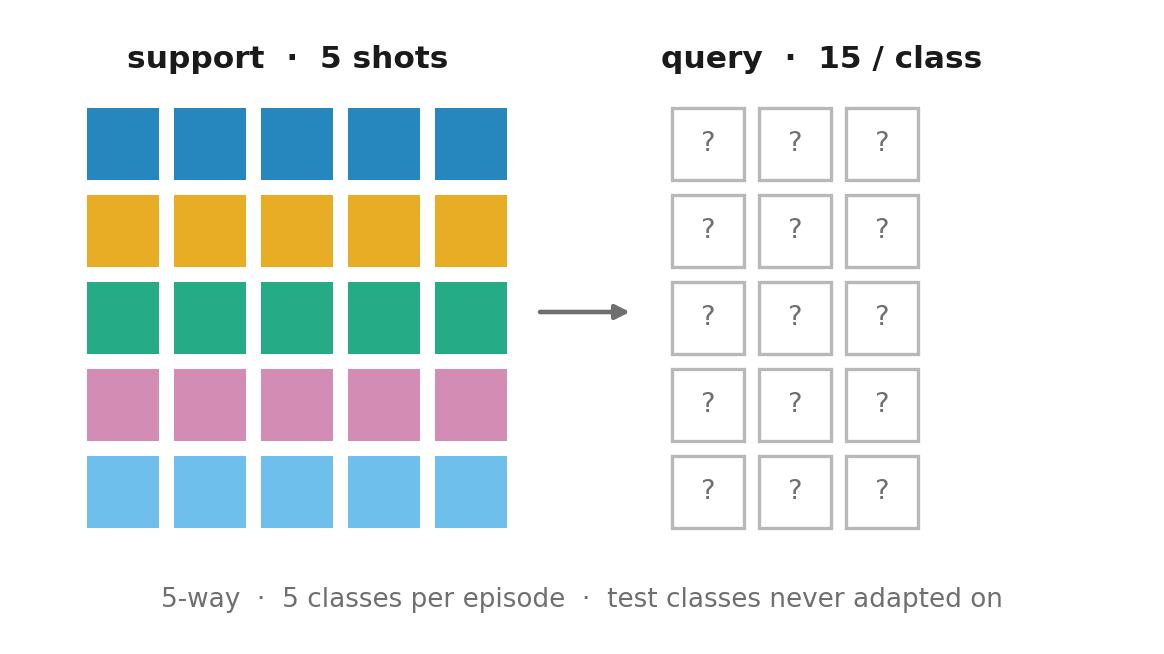
\includegraphics[width=0.6\textwidth]{F2_few_shot_episode_compact.png}
\caption{One 5-way 5-shot episode: five labelled support images per class, and fifteen query images per
class to classify. Test episodes draw their classes only from the 20 test classes.}
\label{fig:episode}
\end{figure}

\begin{itemize}
\item \textbf{Task format.} Each episode samples 5 classes, $K \in \{1, 5\}$ support images per class
and 15 query images per class, giving 75 queries per episode.
\item \textbf{Test episodes.} 600 test episodes are generated from fixed seeds (0--599), stored in the
repository and never changed, so every reported number is computed on exactly the same episodes.
\item \textbf{Validation episodes.} 100 episodes from the validation classes, with their own fixed
seeds (10000--10099), are used for early stopping and for every quantity fitted after training
(temperature scaling and the RQ4 refit). The test episodes are used only for final reporting.
\item \textbf{Training seeds.} Each configuration is trained three times, with seeds 42, 43 and 44. The
stream of training episodes is the same for all seeds, so the seed changes only the random
initialisation of the adapter. We report the mean over the three seeds and use the spread across seeds
to judge whether two configurations really differ.
\end{itemize}

\section{Evaluation Metrics}
\label{sec:metrics}

\subsection{Accuracy and macro-F1}

Top-1 accuracy and macro-averaged F1 are computed per episode and averaged over the 600 test episodes.
In balanced 5-way episodes the two track each other closely.

\subsection{Calibration}

The expected calibration error groups predictions into $M = 15$ equal-width confidence bins
$B_1, \dots, B_M$ and averages the gap between each bin's accuracy and its mean confidence, weighted by
the bin's share of the $n$ predictions:
\begin{equation}
\mathrm{ECE} = \sum_{m=1}^{M} \frac{|B_m|}{n} \,\bigl|\mathrm{acc}(B_m) - \mathrm{conf}(B_m)\bigr| .
\label{eq:ece}
\end{equation}
Our main calibration number is the \emph{pooled} ECE, computed over all 45{,}000 query predictions of
the 600 episodes together. We also report the per-episode ECE (computed on each episode's 75 queries and
then averaged, which is noisier) and the multi-class Brier score,
\begin{equation}
\mathrm{BS} = \frac{1}{n}\sum_{i=1}^{n}\sum_{k=1}^{K}\bigl(\hat p_{i,k} - y_{i,k}\bigr)^2 ,
\end{equation}
a proper scoring rule that uses the whole predicted distribution. For softmax models we also report ECE
after temperature scaling~\cite{guo2017calibration}, with the temperature fitted on the validation
episodes.

\subsection{OOD detection}

In each test episode the 75 in-distribution queries and the 500 images of an OOD set are scored against
that episode's five prototypes with a chosen uncertainty score (\cref{sec:scores}). The area under the
ROC curve (AUROC) measures how well the score separates the two groups: it is the probability that a
randomly chosen OOD image is rated more uncertain than a randomly chosen in-distribution query. We also
report the false-positive rate at 95\% true-positive rate (FPR@95), the fraction of OOD images still
accepted when the threshold keeps 95\% of the in-distribution queries. Both are averaged over the 600
episodes. Higher AUROC and lower FPR@95 are better.

\subsection{Efficiency}

We report the number of trainable parameters and the inference latency per image, measured on a single
CPU thread (median over repeated runs) as a proxy for constrained hardware.
